\documentclass[xelatex,ja=standard,a4paper,10pt,twocolumn]{bxjsarticle}
\geometry{margin=18mm,top=20mm,bottom=22mm,columnsep=7mm}
\usepackage{amsmath,amssymb,mathtools,bm}
\usepackage{graphicx}
\usepackage{booktabs}
\usepackage{multirow}
\usepackage{tabularx}
\usepackage{array}
\usepackage{siunitx}
\usepackage{xcolor}
\usepackage{tikz}
\usetikzlibrary{arrows.meta,positioning,fit,shapes.geometric}
\usepackage{enumitem}
\usepackage{caption}
\usepackage{subcaption}
\usepackage{float}
\usepackage{placeins}
\usepackage{url}
\usepackage[
  colorlinks=true,
  linkcolor=blue!45!black,
  citecolor=blue!45!black,
  urlcolor=blue!55!black
]{hyperref}
\ifpTeX
  \usepackage{pxjahyper}
\fi
\usepackage[nameinlink,noabbrev]{cleveref}

\captionsetup{font=small,labelfont=bf}
\setlength{\emergencystretch}{2em}
\setlength{\parindent}{1em}
\setlength{\parskip}{0pt}
\setlist{nosep,leftmargin=1.8em}
\sisetup{
  detect-all,
  group-separator={,},
  group-minimum-digits=4,
  range-phrase={--},
  range-units=single
}

\newcommand{\pt}{p_{\mathrm{T}}}
\newcommand{\met}{E_{\mathrm{T}}^{\mathrm{miss}}}
\newcommand{\Htt}{H\rightarrow\tau^{+}\tau^{-}}
\newcommand{\Ztt}{Z\rightarrow\tau^{+}\tau^{-}}
\newcommand{\epssig}{\varepsilon_{\mathrm{sig}}}
\newcommand{\epsbkg}{\varepsilon_{\mathrm{bkg}}}
\DeclareSIUnit{\GeV}{GeV}
\DeclareSIUnit{\TeV}{TeV}
\newcommand{\code}[1]{\texttt{\detokenize{#1}}}
\newcommand{\todo}[1]{\textcolor{red!70!black}{[要確認: #1]}}

\crefname{figure}{図}{図}
\crefname{table}{表}{表}
\crefname{section}{節}{節}
\crefname{equation}{式}{式}

\hypersetup{
  pdftitle={再構成されたタウ対による等質量H/Z分離の探索},
  pdfauthor={Ryunosuke Baba}
}


\begin{document}

\twocolumn[
\begin{center}
  {\LARGE\bfseries
    再構成された \(\tau^{+}\tau^{-}\) 系による\\
    等質量 \(H/Z\) 分離の探索\par}
  \vspace{0.6em}
  {\large
    親ボソン横運動量を整合したATLAS高速シミュレーションに対する
    Transformer解析\par}
  \vspace{1.0em}
  {\large Ryunosuke Baba\par}
  \vspace{0.2em}
  {\small ICEPPサマースクール実習レポート\par}
  \vspace{0.2em}
  {\small 2026年7月30日\par}
\end{center}

\begin{minipage}{0.94\textwidth}
\small
\textbf{要旨}\quad
質量差を用いずに \(\Htt\) と \(\Ztt\) を分離できるかを調べるため、
両親粒子の質量を約 \(\SI{91.2}{\GeV}\) に揃えた
hadronic-\(\tau\)候補を含むMonte Carlo事象を解析した。
ATLAS高速シミュレーションを通した修正版sampleのうち、
2026年7月29日時点で利用可能であった63.1\%を固定snapshotとし、
同一の再構成およびevent selectionを適用した。
選択後、train、validation、testを先に固定し、各split内でtruth親ボソン
\(\pt\) を \(\SI{20}{\GeV}\) binごとにH/Z同数へdownsampleした。
これにより、親\(\pt\) だけをscoreとしたAUCは
\(0.5705\)から\(0.5007\)へ低下した。

再構成された\(\tau\)、track、particle-flow object、missing transverse
momentumを可変長token列として表し、bidirectional Transformerで分類した。
validationだけでハイパーパラメータとepochを固定した最終モデルは、
56,338 test事象に対してROC AUC \(0.6088\)、binary cross entropy
\(0.6749\)を得た。test ROC上で信号効率\(0.7000\)となる点の背景効率は
\(0.5490\)、背景除去率は\(1.8216\)であった。ここで「背景」は
分類問題のZ classだけを指し、jetやtop backgroundを含まない。
これは、質量と親\(\pt\)を制御した後にも再構成量にラベル依存情報が残る
ことを示す。ただし、入力はスピン観測量だけに限定されず、親\(\pt\)以外の
生成・再構成差、統計誤差および系統誤差の評価も残っている。
したがって、本結果はスピン相関を単独で測定したものではなく、
再構成レベルでの分離可能性を示すproof of conceptである。
\end{minipage}
\vspace{1.2em}
]

\section{序論}
\label{sec:introduction}

\(\tau\) leプトンは寿命が短く、検出器内で直接観測される前に崩壊する。
一方で、その崩壊粒子の運動学分布は親\(\tau\)の偏極に依存する。
したがって、\(\tau^{+}\tau^{-}\)対の崩壊生成物を組み合わせれば、
対を生成した粒子のスピンおよび結合構造へ感度を持ち得る
\cite{TauSpinner,TauSpinML}。
この性質は、scalarであるHiggs bosonとvector bosonである\(Z\)を
\(\tau\tau\)終状態で比較する動機になる。

通常のStandard Model \(H\) と \(Z\) では質量が大きく異なるため、
再構成量を用いた分類器は、スピン相関を使わずとも質量やそれと相関する
運動学量から両者を分離できる。本研究ではこの自明な差を抑えるため、
Higgs-like scalar \(H\) と\(Z\)の生成質量をともに約
\(\SI{91.2}{\GeV}\)へ設定した専用Monte Carlo sampleを用いる。
これは\(\SI{125}{\GeV}\)のStandard Model Higgs bosonを測定する解析ではなく、
ほぼ同じ質量を持つscalar-like sampleとvector \(Z\) sampleの比較である。
さらに、初期診断で残っていた親ボソン\(\pt\)分布の差を取り除くため、
truth情報を用いてH/Zの\(\pt\)分布を揃える。

この条件の下で、再構成されたhadronic-\(\tau\)候補と、そのtrack、
neutral/PFO、eventの\(\met\)をTransformer
\cite{Transformer}へ入力する。Transformerは可変長の構成要素を
同一event内で直接関連付けられるため、固定長の高レベル変数へ情報を
圧縮せずに、\(\tau\)崩壊の多次元相関を扱える。

本稿では、まず使用したsampleと再構成を\cref{sec:samples}で述べる。
\cref{sec:method}では\(\pt\) matching、入力表現、学習とモデル選択を
定義し、\cref{sec:results}で最終性能を示す。
最後に\cref{sec:discussion}で、結果から言えることと、スピン相関へ
帰属する前に必要な検証を分けて議論する。

\section{Monte Carlo sampleと事象再構成}
\label{sec:samples}

\subsection{専用 \(H/Z\rightarrow\tau\tau\) sample}

入力は、\(H+j\)および\(Z+j\)生成と\(\tau\)崩壊を分けて作り、
Les Houches Eventを結合した専用sampleである。
重心系エネルギーは\(\sqrt{s}=\SI{13}{\TeV}\)である。
production過程にはMadGraph 3.5.5
\cite{MadGraph5}、parton showerにはPythia 8.312
\cite{Pythia82}、heavy-flavour decayにはEvtGen 2.2.1を用いた。
ntupleで確認したtruth親ボソン質量は、H sampleが
\(\SI{91.1872}{\GeV}\)、Z sampleが\(\SI{91.1876}{\GeV}\)であり、
解析の目的に対して同一質量とみなせる設定である。
production側にはpartonの\(\pt>\SI{200}{\GeV}\)という生成条件がある。
\(\tau\)崩壊はTauDecay UFOを用いて行い、生成段階のスピン相関を
崩壊粒子へ伝える構成とした。

検出器応答にはATLASのAtlFast3
\cite{ATLASDetector,AtlFast3}を用いた。
入力metadataは\code{ATLFAST3_QS}、campaignは\code{mc20e}、
AMI tagは\code{r14861}である。再構成後の入力形式は
\code{DAOD_PHYS}である。private production directoryでは999801と999802を
sample識別子として用いたが、これらを公式DSIDとはみなさない。
ntupleの\code{mcChannelNumber}は両sampleとも999999であり、
H/Zはsample名とtruth親ボソンPDG ID 25/23で監査した。
parton distribution functionとtuneは固定snapshotのmetadataから
追跡できなかったため、本稿では断定しない。

sample全体の生成完了を待たず、2026年7月29日21時59分時点で
正常に開けたDAODを\code{fixed-partial-v2}として凍結した。
予定していたH/Z各500 fileに対し、Hは331 file、Zは300 fileであり、
全体の63.1\%に相当する。Hの1 fileは生成途中でcloseされておらず、
ROOTで開けなかったため除外した。
\cref{tab:sample_counts}に入力数とevent selection後の数を示す。
全64 HTCondor jobはreturn code 0で完了し、出力64 ROOT fileは
すべて読み取り可能であった。H/Zで84 branchのschemaが一致し、
truth親ボソンPDG IDの不一致は0であった。

\begin{table*}[t]
  \centering
  \caption{固定snapshot \code{fixed-partial-v2}のevent数。
    selection効率はselected entryを実際に読み取れたraw event数で割った値である。}
  \label{tab:sample_counts}
  \begin{tabular}{lrrrrr}
    \toprule
    sample & private ID & DAOD file & raw event & selected event & selection効率 \\
    \midrule
    \(H\rightarrow\tau\tau\) & 999801 & 331 & 661,964 & 332,932 & 50.29\% \\
    \(Z\rightarrow\tau\tau\) & 999802 & 300 & 599,955 & 306,731 & 51.13\% \\
    \midrule
    合計 & --- & 631 & 1,261,919 & 639,663 & 50.69\% \\
    \bottomrule
  \end{tabular}
\end{table*}

\subsection{\(\tau\)候補とevent selection}
\label{subsec:selection}

再構成にはAnalysisBase 25.2.32のCommon Physics処理を用いた。
\code{TauJets}から解析用copyを作り、energy calibrationとselectionを
H/Zへ共通に適用した。hadronic-\(\tau\)の再構成と同定の一般的な考え方は
Ref.~\cite{ATLASTauID}にまとめられている。
本解析の具体的なselectionを\cref{tab:selection}に示す。
条件を通る候補がちょうど2本で、かつopposite-signであるeventだけを残した。
出力では負電荷側を\(\tau_0=\tau^-\)、正電荷側を
\(\tau_1=\tau^+\)とする。
truth matchingまたはtruth hadronic-decay flagはselectionに要求せず、
trigger requirementも設けていない。

\begin{table}[t]
  \centering
  \caption{解析に用いた\(\tau\)候補およびevent selection。}
  \label{tab:selection}
  \small
  \begin{tabular}{ll}
    \toprule
    項目 & 条件 \\
    \midrule
    入力container & \code{TauJets} \\
    \(\tau\) transverse momentum & \(\pt\geq\SI{20}{\GeV}\) \\
    \(\tau\) pseudorapidity & \(|\eta|\leq 2.5\) \\
    \(\tau\) charge & \(|q|=1\) \\
    track multiplicity & 1または3 \\
    jet rejection & RNN Loose \\
    \(\eta\) crack veto & なし \\
    \(\phi\) requirement & なし \\
    candidate multiplicity & 条件通過候補がちょうど2本 \\
    pair charge & opposite-sign \\
    \bottomrule
  \end{tabular}
\end{table}

入力DAODにはGNTau v0のscoreとflagが保存されていたが、
AnalysisBase 25.2.32の標準GNTau selectionが要求する
\code{GNTauL_v1trunc}とは互換でなかった。そのため、GNTau flagを
標準Loose selectionと同一視せず、本解析のselectionにはRNN Looseを使った。
GNTau/RNNの連続scoreは診断用branchとして保存し、一部はNN入力へ用いた。

入力DAODには保存済みFinal \(\met\) termがなかった。
そこで、\code{MET_Core_AntiKt4EMPFlow}、
\code{METAssoc_AntiKt4EMPFlow}および較正済みのelectron、muon、
photon、jet、\(\tau\)を用いて、CPのMissingET blockから
\code{AnaMET_NOSYS["Final"]}を再構成した。
標準Overlap Removalも同時に実行した。
処理はnominal-onlyで、object efficiency scale factorとsystematic
variationは適用していない。
FastSim専用のtau smearing recommendationがない補正については、
FullSim recommendationへfallbackするwarningが記録された。

\subsection{解析ntuple}

自作の\code{TauSpinNtupleAlg}は、selectionを通過した1 eventを
TTree \code{tauspin}の1 entryとして保存する。eventおよびFinal \(\met\)、
2本の\(\tau\) summary、各\(\tau\)に対応する可変長trackとPFO、
vertex、truth診断を合わせて84 branchを持つ。
truth branchはsample監査、親\(\pt\) matchingおよびlabel確認に使うが、
分類器の入力には使わない。

固定snapshotのntuple生成では全jobが終了したものの、MetMakerから
soft termに重複する可能性のあるobjectがmissingである旨のmessageが
20 jobに計24行記録された。また、全64 jobでinvalidなtau-track linkを
skipした旨のwarningが少なくとも1回記録されており、event単位の発生頻度は
監査していない。これらはjobの失敗や非有限なFinal \(\met\)には
直結しなかったが、
保存済みFinal \(\met\)を持つ標準DAODとの数値比較は未実施である。
この点は最終的なdetector-level性能を解釈する際の制約として残す。

\section{解析手法}
\label{sec:method}

\subsection{データ分割と親ボソン \(\pt\) matching}
\label{subsec:matching}

H/Zのntupleを、決定的hashによりtrain、validation、testへ
80:10:10で先に分けた。同じsample内で\code{eventNumber}が重複したため、
hash keyにはsample名、ROOT basename、file-local entry indexを用いた。
この定義は同じfile構成からは再現するが、ROOT fileを再chunkまたは
再mergeすると変化し得る。

分割後、それぞれのsplit内でtruth親ボソン\(\pt\)を
\(\SI{20}{\GeV}\)幅に分けた。\(\SI{1000}{\GeV}\)以上は1個の
overflow binとした。split \(s\)、bin \(i\)で保持するH/Z event数を
\begin{equation}
  N^{\mathrm{keep}}_{s,i}
  = \min\left(N^{H}_{s,i},N^{Z}_{s,i}\right)
  \label{eq:pt_matching}
\end{equation}
とし、seed 42で各classから固定downsamplingした。
この順序により、同一eventが複数splitへ移ることなく、各split内で
H/Zの親\(\pt\)分布を揃えた。

\cref{tab:split_counts}にmatching前後のevent数を示す。
全体の保持率はHで85.62\%、Zで92.93\%であった。
親\(\pt\)そのものをclassifier scoreとしたROC AUCは、
matching前の0.570524からmatching後の0.500660へ低下した。
したがって、少なくとも親\(\pt\)の1次元分布だけによる直接的な
label識別はほぼ除かれている。

\begin{table*}[t]
  \centering
  \caption{deterministic splitとtruth親ボソン\(\pt\) matching前後のevent数。}
  \label{tab:split_counts}
  \begin{tabular}{lrrrrrr}
    \toprule
    & \multicolumn{3}{c}{matching前} & \multicolumn{3}{c}{matching後} \\
    \cmidrule(lr){2-4}\cmidrule(lr){5-7}
    split & H & Z & 合計 & H & Z & 合計 \\
    \midrule
    train      & 266,685 & 245,519 & 512,204 & 228,360 & 228,360 & 456,720 \\
    validation &  33,312 &  30,693 &  64,005 &  28,519 &  28,519 &  57,038 \\
    test       &  32,935 &  30,519 &  63,454 &  28,169 &  28,169 &  56,338 \\
    \midrule
    合計       & 332,932 & 306,731 & 639,663 & 285,048 & 285,048 & 570,096 \\
    \bottomrule
  \end{tabular}
\end{table*}

\subsection{入力表現と前処理}
\label{subsec:features}

入力eventを次の可変長token列へ変換した。
\begin{equation}
\begin{split}
  [\mathrm{CLS}], [\mathrm{EVENT}],&
  [\tau^-], [\mathrm{TRACK}^- \ldots], [\mathrm{PFO}^- \ldots],\\
  &[\tau^+], [\mathrm{TRACK}^+ \ldots], [\mathrm{PFO}^+ \ldots].
\end{split}
\label{eq:token_sequence}
\end{equation}
trackとPFOは各\(\tau\)側で\(\pt\)降順に並べた。
eventごとにtoken数が異なるため、保存時はpaddingせず、
mini-batch内の最大長までdynamic paddingし、padding maskを用いた。

入力の概要を\cref{tab:features}に示す。
Relative-v3表現では、絶対的な再構成量に加え、track/PFOと親\(\tau\)の
相対座標、\(\tau\)対の相対量、各\(\tau\)と\(\met\)の角度差を加えた。
truth量、sample識別子、event/run番号、primary vertex座標は入力から除いた。

\begin{table*}[t]
  \centering
  \caption{Relative-v3のtoken別入力。次元は前処理後に各projectorへ渡す
    連続特徴量の数であり、decay-mode categoryは別embeddingで加える。}
  \label{tab:features}
  \small
  \begin{tabularx}{\textwidth}{@{}l c X@{}}
    \toprule
    token & 次元 & 主な入力 \\
    \midrule
    EVENT & 13 &
      Final \(\met\)、\(\phi(\met)\)、sum \(E_{\mathrm{T}}\)、
      \(\tau\)対の\(|\Delta\eta|\)、\(\sin/\cos\Delta\phi\)、
      \(\log(\pt^{\tau^-}/\pt^{\tau^+})\)、
      \(\met\)と各\(\tau\)の\(\sin/\cos\Delta\phi\)、
      \(\met/(\pt^{\tau^-}+\pt^{\tau^+})\) \\
    TAU & 10 &
      \(\pt,\eta,\phi,m\)、track数、isolation track数、
      RNN/GNTau score、vertex \(\Delta z\)。
      decay modeはcategory embedding \\
    TRACK & 19 &
      \(\pt,\eta,\phi,q,d_0,z_0\sin\theta\)、track分類flag、
      Pixel/SCT/TRT hit数、親\(\tau\)に対する
      \(\Delta\eta,\sin/\cos\Delta\phi,\log(1+\pt\mathrm{\ fraction})\) \\
    PFO & 10 &
      \(\pt,\eta,\phi,E\)、\(\pi^0\) flag、親\(\tau\)に対する
      \(\Delta\eta,\sin/\cos\Delta\phi,\log(1+\pt\mathrm{\ fraction})\) \\
    \bottomrule
  \end{tabularx}
\end{table*}

\(\phi\)は\(\sin\phi,\cos\phi\)へ変換した。
\(\pt\)、energy、mass、\(\met\)、sum \(E_{\mathrm{T}}\)は
\(\log(1+x/\SI{1}{\GeV})\)へ写し、その後に標準化した。
その他の連続量も必要に応じて標準化した。
平均と標準偏差はtrain splitだけから計算し、validation/testの情報を
前処理へ混ぜていない。全570,096 eventについて、Tensorのfinite値、
label、offset終端、shard内event数を検証した。

\begin{figure*}[t]
  \centering
  \resizebox{0.98\textwidth}{!}{%
  \begin{tikzpicture}[
    node distance=8mm and 8mm,
    box/.style={
      draw=black!65, rounded corners=2pt, align=center,
      minimum height=10mm, text width=29mm, fill=blue!4
    },
    decision/.style={
      draw=black!65, rounded corners=2pt, align=center,
      minimum height=10mm, text width=31mm, fill=orange!8
    },
    arrow/.style={-{Latex[length=2.4mm]},thick,draw=black!65}
  ]
    \node[box] (daod) {専用 \(H/Z+j\)\\DAOD\_PHYS\\mass \(\simeq\SI{91.2}{\GeV}\)};
    \node[box,right=of daod] (reco) {共通CP再構成\\RNN Loose\\exactly 2 OS \(\tau\)};
    \node[box,right=of reco] (split) {deterministic\\80:10:10 split};
    \node[decision,right=of split] (match) {split内truth \(\pt\)\\20 GeV-bin matching};
    \node[box,right=of match] (tokens) {Relative-v3\\可変長token列\\dynamic padding};
    \node[box,right=of tokens] (model) {bidirectional\\Transformer\\\(H=1,\ Z=0\)};
    \node[decision,right=of model] (select) {validation-only\\HPO・epoch選択};
    \node[box,right=of select] (test) {固定modelの\\test評価\\AUC \(=0.6088\)};

    \draw[arrow] (daod) -- (reco);
    \draw[arrow] (reco) -- (split);
    \draw[arrow] (split) -- (match);
    \draw[arrow] (match) -- (tokens);
    \draw[arrow] (tokens) -- (model);
    \draw[arrow] (model) -- (select);
    \draw[arrow] (select) -- (test);
  \end{tikzpicture}}
  \caption{解析の全体フロー。truth親ボソン\(\pt\)はmatchingにのみ使い、
    Transformerへは入力しない。ハイパーパラメータと最終epochは
    validationだけで固定してから、最終モデルをtestへ適用した。}
  \label{fig:workflow}
\end{figure*}

\subsection{Transformerと学習}

EVENT、TAU、TRACK、PFOには別々のlinear projectorを用い、
すべてを\(d_{\mathrm{model}}=128\)次元へ写した。
これにobject-type embedding、\(\tau\)-side embedding、
\(\tau\) decay-mode embeddingを加えた。
通常のsequence positional encodingは使用しない。
encoderはbidirectionalであり、causal maskも用いない。

最終的に選ばれたCurrent profileは、8 attention heads、
4 encoder layers、feed-forward dimension 512、GELU、
pre-layer normalizationからなる。
\([\mathrm{CLS}]\)の最終hidden stateを2層MLPへ入力し、
\(H=1\)、\(Z=0\)の1 logitを出力する。trainable parameter数は819,201である。

lossには\code{BCEWithLogitsLoss}を用い、trainではH/Z balanced
samplingを行った。MC event weightは使用していない。
optimizerはAdamW、weight decay \(10^{-4}\)、batch size 128、
random seed 42とし、TF32で学習した。

\subsection{HPOとモデル選択}
\label{subsec:model_selection}

Optuna \cite{Optuna}を用い、model profile、learning rate、dropout、
schedulerを21 trialで探索した。
探索範囲と選択設定を\cref{tab:hpo}にまとめる。
HPO中はtest splitを読み込まず、full validation AUCだけを用いた。
objectiveはepoch 8以降の連続3 epochのvalidation AUC平均の最大値とし、
最大windowの中央epoch checkpointを保存した。

trial間の途中pruningは使用しなかった。
Relative-v3が遅れて改善する可能性を保つため、各trialは少なくとも
20 epoch実行した。その後、rolling AUCのplateauまたはAUCとlossの
同時悪化に基づくtrial内early stoppingだけを許した。
21 trialはすべて正常終了し、18 trialがearly stopした。

\begin{table}[t]
  \centering
  \caption{HPOの探索範囲と、validation-only規則で選択したtrial 5。}
  \label{tab:hpo}
  \small
  \begin{tabularx}{\columnwidth}{@{}l X l@{}}
    \toprule
    parameter & 探索範囲 & trial 5 \\
    \midrule
    profile & Small/Current/Deep/\newline Wide/Large & Current \\
    learning rate & \(7\times10^{-5}\)--\(2\times10^{-4}\) & \(10^{-4}\) \\
    dropout & 0--0.25 & 0.10 \\
    scheduler & constant/cosine & cosine \\
    warmup & scheduler依存 & 5\% \\
    weight decay & 固定 & \(10^{-4}\) \\
    parameter数 & profile依存 & 819,201 \\
    \bottomrule
  \end{tabularx}
\end{table}

順位は3-epoch平均AUCを主指標とした。首位との差が0.001未満なら
minimum validation loss、さらに同程度ならparameter数の小さい方を
優先した。trial 5のobjectiveは0.604504で、順位規則上の2位trial 13との
差は0.000156にすぎない。したがってtrial 5を唯一の最適点とはみなさず、
21 trialと事前に定めた規則の下で選ばれた設定として扱う。

\begin{figure*}[t]
  \centering
  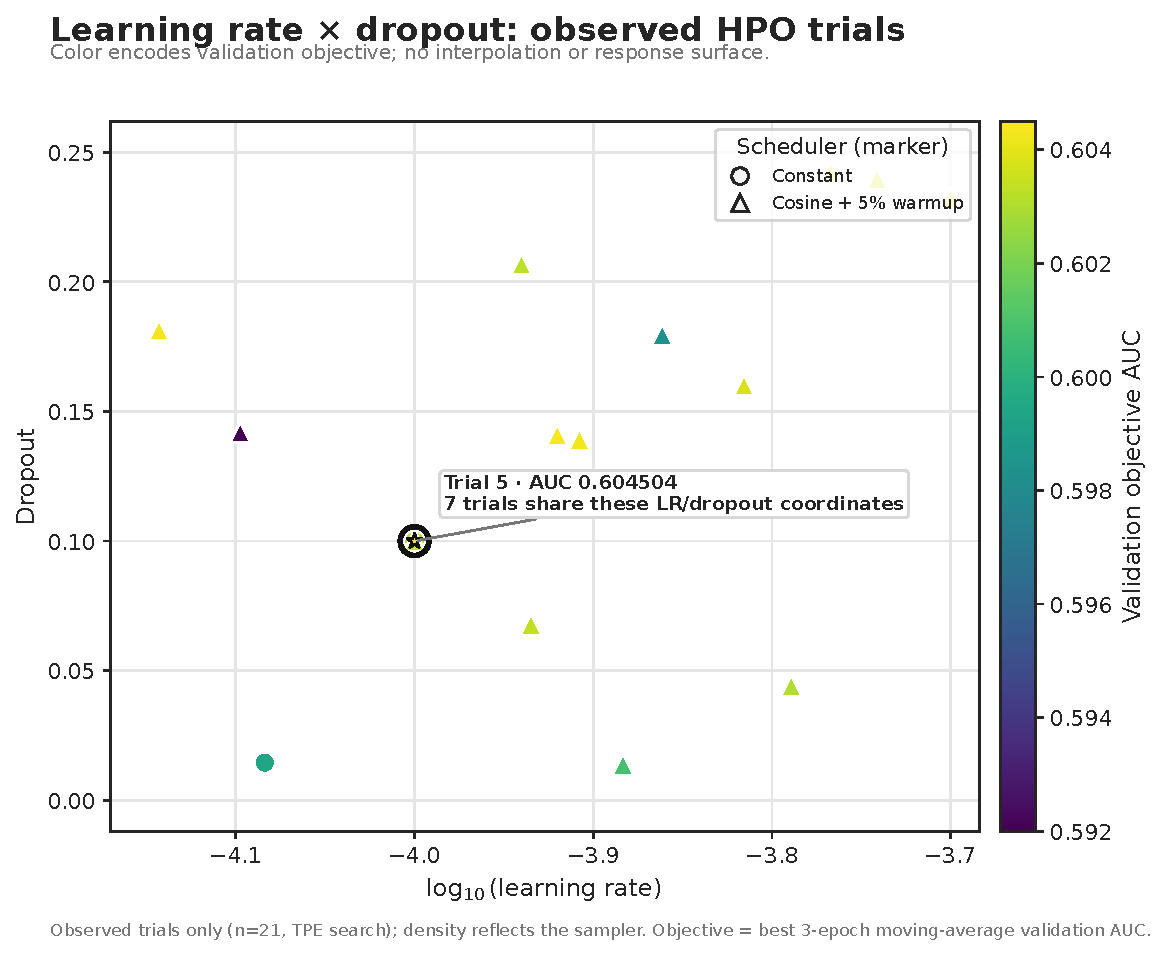
\includegraphics[width=0.78\textwidth]{figures/lr_dropout_objective_scatter.pdf}
  \caption{HPOで実際に評価したlearning rateとdropoutの組。
    色はbest 3-epoch moving-average validation AUC、markerはschedulerを示す。
    星付きの点がtrial 5である。同じ座標に7個のanchor trialが重なっている。
    TPEによる探索点は一様標本ではないため、点密度を性能の確率密度として
    解釈せず、図には補間面も描いていない。}
  \label{fig:hpo}
\end{figure*}

\section{結果}
\label{sec:results}

\subsection{40 epoch最終学習}

HPOで固定したtrial 5の設定を使い、early stoppingを無効にして
40 epochの最終学習を最初から実行した。
cosine schedulerは総step数に依存するため、このrunは32 epochの
HPO checkpointを延長したものではなく、40 epoch horizonを持つ
独立な再学習である。

連続3 epochのvalidation AUC平均はepoch 23--25で最大
0.6044569となった。その中央であるepoch 24を、test評価前に
最終checkpointとして固定した。
epoch 24のvalidation AUCは0.6047115、lossは0.6770760である。

\cref{fig:learning_curve}に学習履歴を示す。
epoch 24から40までtrain lossは0.669320から0.664270へ低下した一方、
validation lossは上昇し、validation AUCも0.6047115から0.602389へ
低下した。trainへの適合だけが進み、未見データの性能が悪化する
3指標の整合した挙動であり、epoch 24以降を過学習と解釈した。

\begin{figure*}[t]
  \centering
  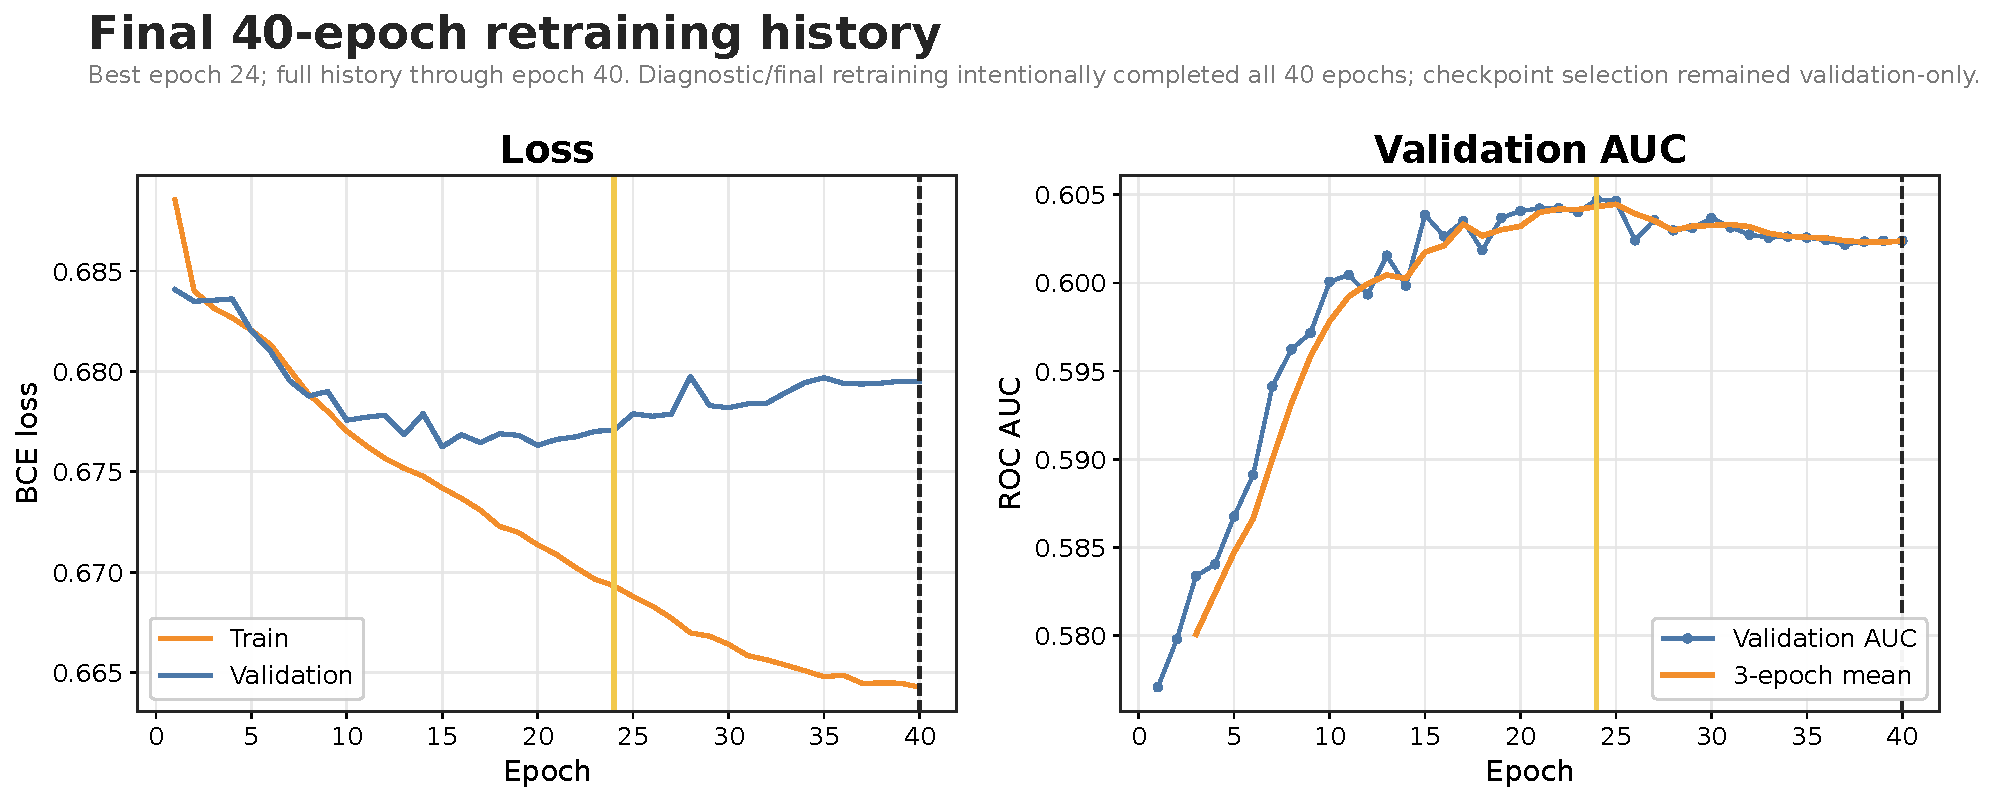
\includegraphics[width=0.94\textwidth]{figures/learning_curve_combined.pdf}
  \caption{trial 5設定を用いた40 epoch最終再学習。
    左はtrain/validation BCE loss、右はvalidation ROC AUCと3-epoch平均。
    黄色線は選択したepoch 24、黒破線は学習終端を表す。
    epoch 24以降、train lossは低下し続ける一方でvalidation lossとAUCが
    悪化しており、過学習が見える。}
  \label{fig:learning_curve}
\end{figure*}

\subsection{最終分類性能}

選択checkpointを再読込し、validation AUCとlossを保存時の値と
差0で再現した。その後、固定した最終モデルをtest splitへ適用した。
結果を\cref{tab:final_metrics}に示す。
test ROC AUCは0.6088142、BCE lossは0.6749150であった。
validationとtestのAUCおよびlossは近く、両splitの間に明らかな
性能不整合は見られない。

\begin{table}[t]
  \centering
  \caption{epoch 24最終モデルのvalidation/test性能。
    70\%信号効率に関する値は、各splitのROC上でその効率に最初に到達する
    点をsplitごとに読み取った記述値である。}
  \label{tab:final_metrics}
  \small
  \begin{tabular}{lrr}
    \toprule
    指標 & validation & test \\
    \midrule
    event数 & 57,038 & 56,338 \\
    ROC AUC & 0.604712 & 0.608814 \\
    BCE loss & 0.677076 & 0.674915 \\
    \(\epssig\) & 0.700025 & 0.700025 \\
    \(\epsbkg=\varepsilon_Z\) & 0.560188 & 0.548972 \\
    \(1/\varepsilon_Z\) & 1.78512 & 1.82159 \\
    \bottomrule
  \end{tabular}
\end{table}

test ROC上で\(\epssig\geq0.70\)を初めて満たす点は、
classifier score threshold 0.465762に対応した。
そのとき\(\epssig=0.700025\)、\(\epsbkg=0.548972\)、
背景除去率\(1/\epsbkg=1.821586\)であった。
ここでsignalはH class、backgroundはZ classであり、この値は
jet、top-quark過程などに対するbackground rejectionではない。
このthresholdはtest scoreから読み取ったものであり、
validationで固定してtestへ移したoperating pointではない。
したがって、本稿ではROC曲線上の記述的な性能点としてのみ扱う。

\begin{figure*}[t]
  \centering
  \begin{subfigure}[t]{0.49\textwidth}
    \centering
    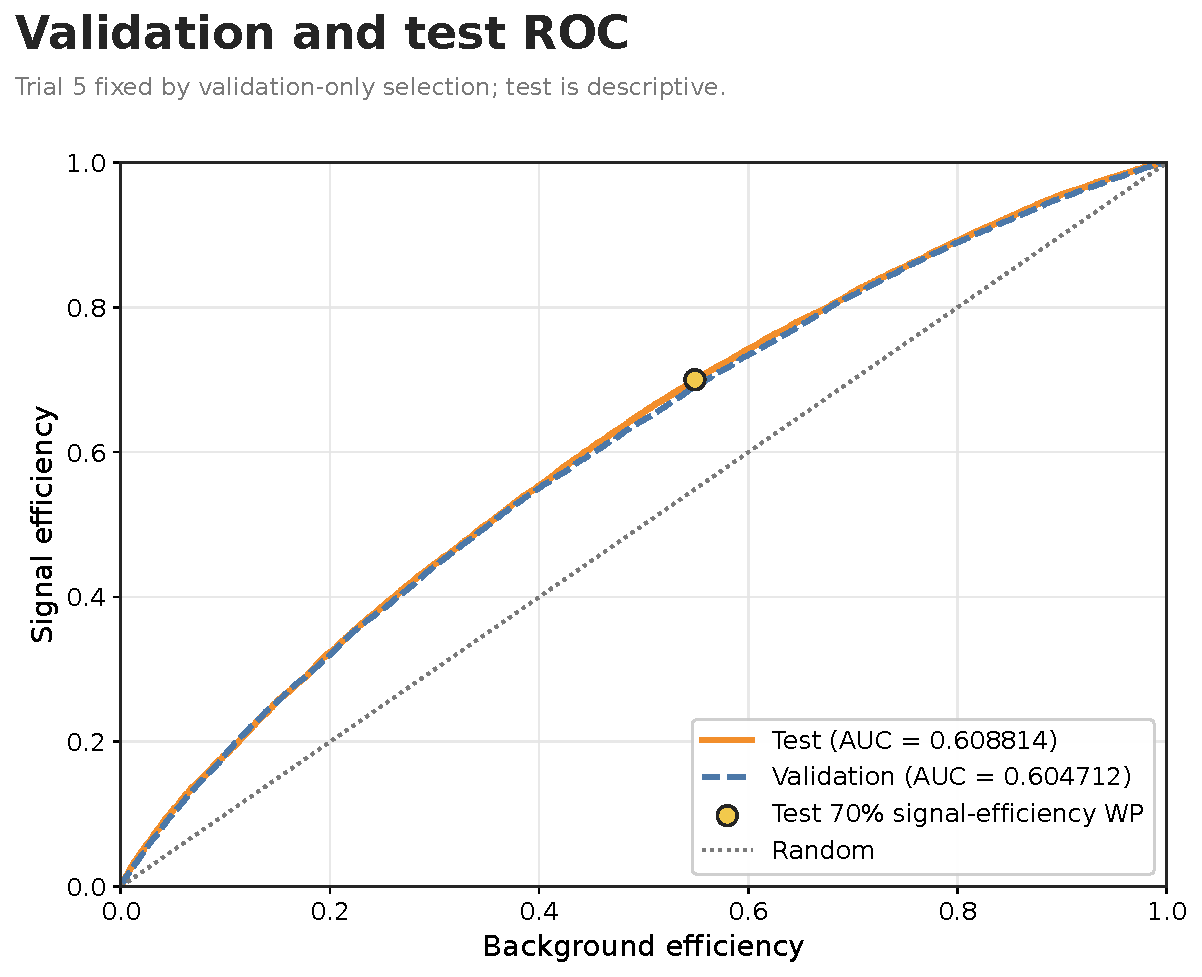
\includegraphics[width=\textwidth]{figures/roc_val_vs_test.pdf}
    \caption{validationおよびtestのROC。}
    \label{fig:roc}
  \end{subfigure}
  \hfill
  \begin{subfigure}[t]{0.49\textwidth}
    \centering
    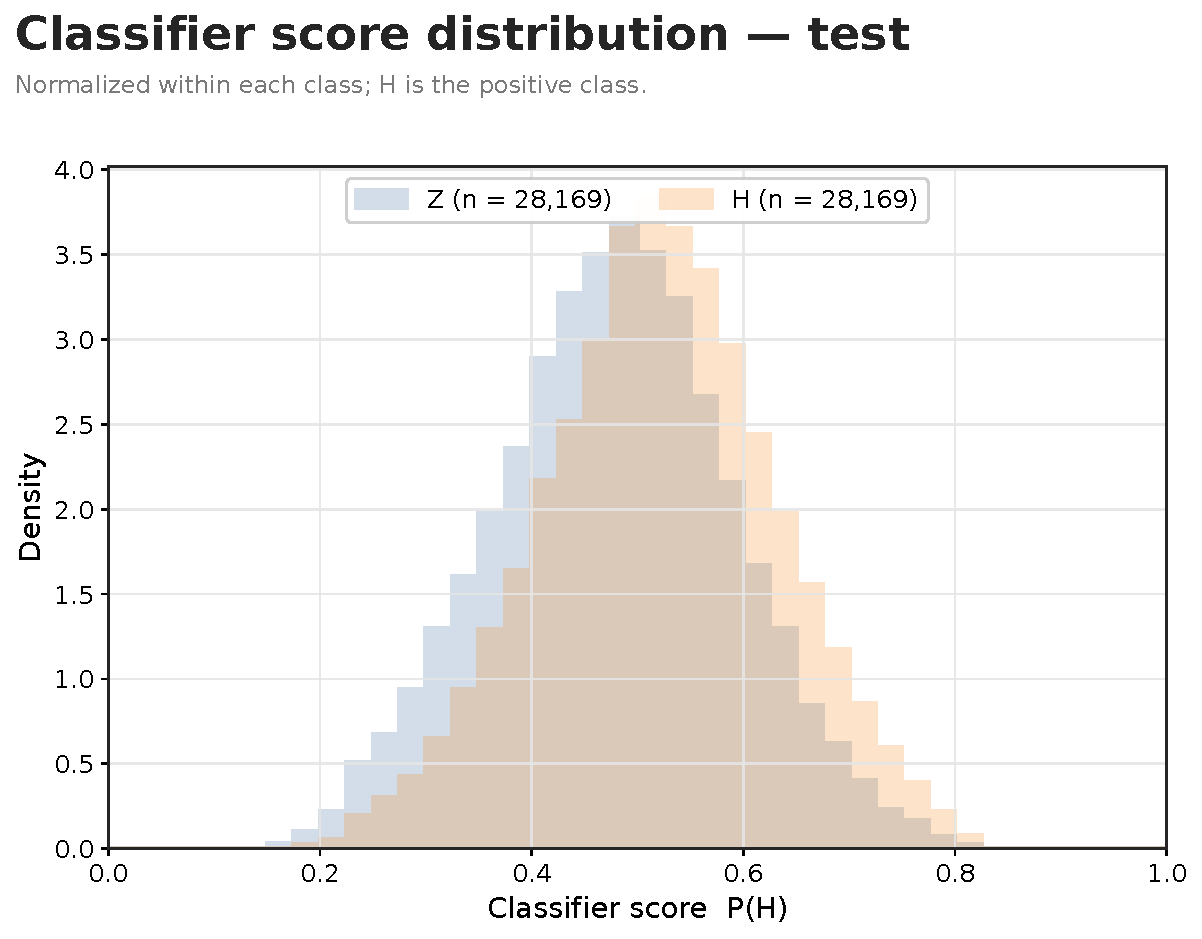
\includegraphics[width=\textwidth]{figures/score_distribution_test.pdf}
    \caption{testにおける\(P(H)\) score分布。}
    \label{fig:scores}
  \end{subfigure}
  \caption{最終モデルの分類性能。H/Zのscore分布は大きく重なるが、
    Hは高score側、Zは低score側へ系統的にずれ、AUCは0.5を上回る。
    左図の70\%信号効率点はtest ROC上で読み取った記述点である。}
  \label{fig:classification}
\end{figure*}

\subsection{親ボソン \(\pt\) 依存性}

\cref{fig:pt_auc}にtest AUCのtruth親ボソン\(\pt\)依存性を示す。
中央領域ではmatchingに用いた\(\SI{20}{\GeV}\) binを保ち、
低統計となる\(\pt<\SI{180}{\GeV}\)と
\(\pt\geq\SI{460}{\GeV}\)はそれぞれ統合した。
error barはclass-stratified bootstrapを1000回行った
16--84 percentile区間であり、有限test sampleによる統計変動の目安である。

多くのbinでAUCはおよそ0.59--0.63に分布し、
親\(\pt\)に対する単調な増減は見られない。
\(\pt<\SI{180}{\GeV}\)ではAUCが0.5528と低い一方、
高\(\pt\)側はevent数が少なく区間も広い。
bin間の差に対するlook-elsewhere効果やsystematic uncertaintyは
評価していないため、局所的な上下を物理効果として解釈しない。

\begin{figure*}[t]
  \centering
  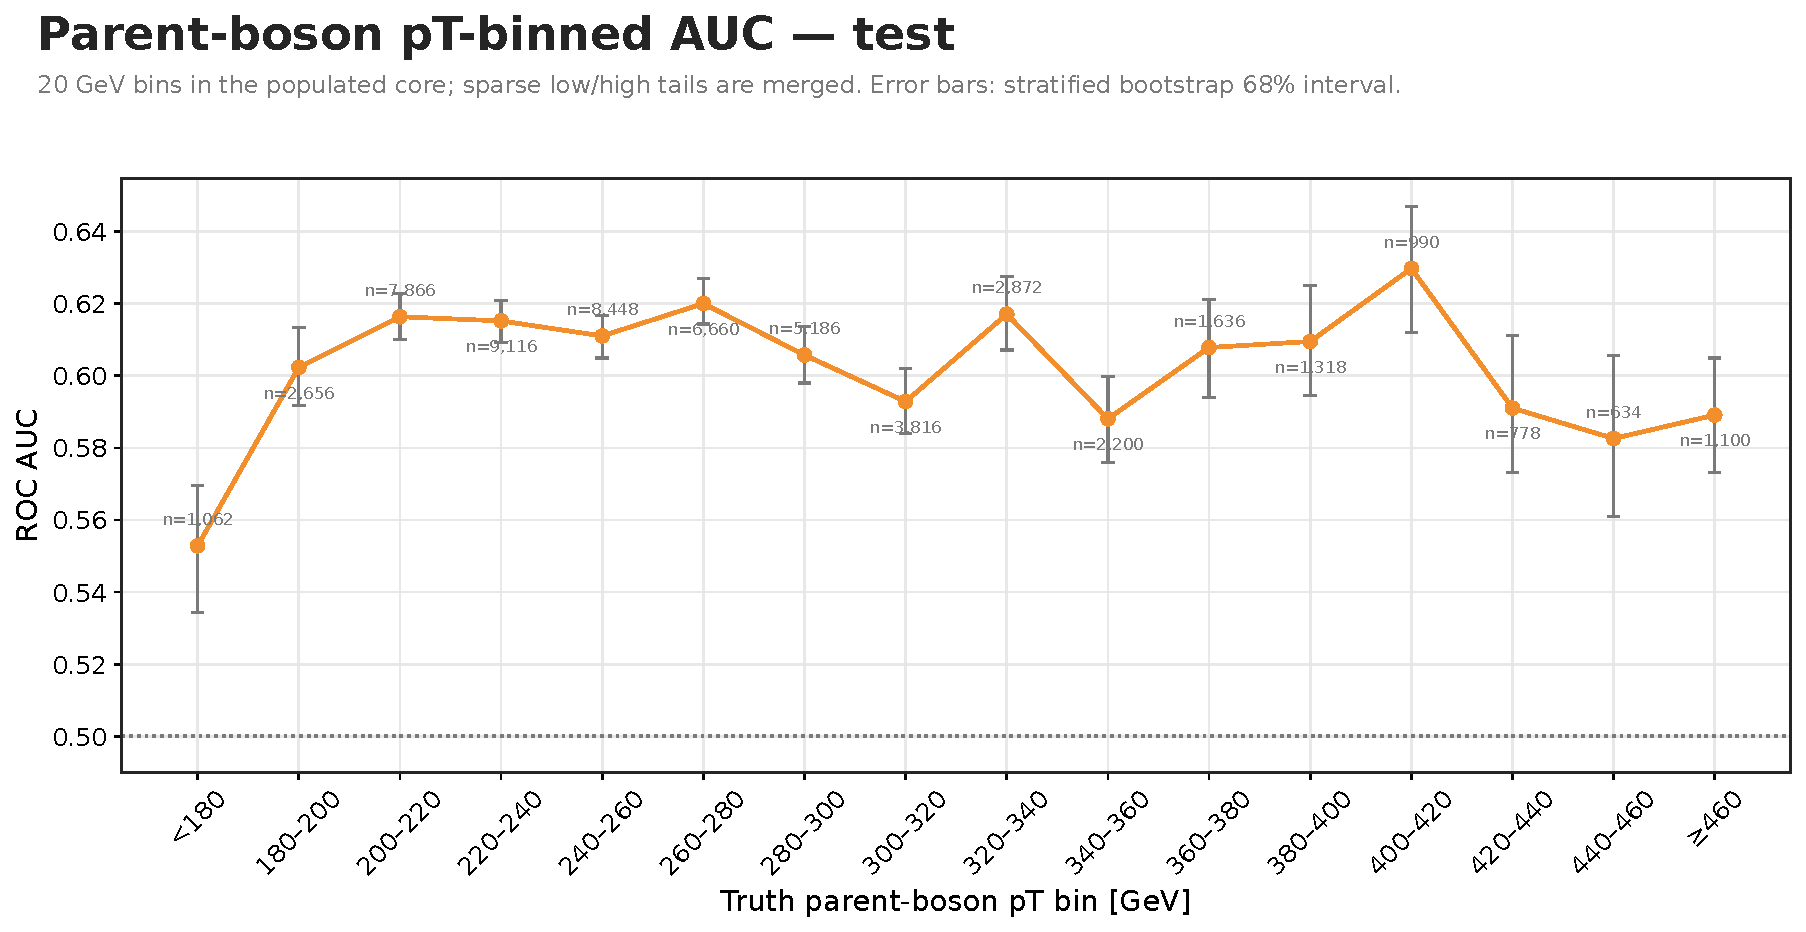
\includegraphics[width=0.78\textwidth]{figures/pt_binned_auc_test.pdf}
  \caption{truth親ボソン\(\pt\) binごとのtest ROC AUC。
    H/Z event数は各binで等しい。error barはclass-stratified bootstrap
    1000回による68\%区間であり、systematic uncertaintyではない。
    低・高\(\pt\)の疎なtailは統合している。}
  \label{fig:pt_auc}
\end{figure*}

\section{物理解釈と解析上の制約}
\label{sec:discussion}

\subsection{結果が示すこと}

親ボソンの質量は生成段階で揃え、さらにtruth親\(\pt\)を各split内で
H/Z同分布にした。matching後の\(\pt\)-only AUCは0.5007まで低下したため、
最終AUC 0.6088を質量差または親\(\pt\)の1次元分布だけで説明することは
できない。再構成された\(\tau\)の運動学、崩壊構成要素、impact parameter、
ID score、\(\met\)およびそれらの相対量には、H/Z labelと相関する
多次元情報が残っている。

\(\tau\)崩壊粒子の分布が偏極とspin correlationを解析することは
よく知られており\cite{TauSpinner,TauSpinML}、本結果の一部がその情報に
由来することは物理的に期待できる。しかし、今回のclassifierは
理論的に定義されたspin observableだけを入力していない。
したがって、AUC 0.6088を「spinだけによる分離能」と同一視することは
できない。より正確には、\emph{質量と親\(\pt\)を制御した専用sampleにおいて、
広い再構成情報を使うTransformerがH/Zを統計的に分離した}、と結論する。

\subsection{統計・系統誤差}

本解析ではinclusive AUC、BCE loss、背景除去率に対する統計区間を
評価していない。示したbootstrap区間は\(\pt\)-bin AUCだけを対象とする。
また、detector calibration、tau ID、track/PFO、MET、pile-up、
generator、shower、PDFなどのsystematic variationも処理していない。
object efficiency scale factorとMC event weightも使用していない。
H/Zは等数へdownsampleしたunweighted classとして扱っており、
cross section、integrated luminosity、期待event yield、significanceは
計算していない。
よって、数値は特定のnominal Monte Carlo sampleに対するclassifier性能であり、
実データ解析の期待感度または測定精度ではない。

\subsection{sampleとvalidation上の制約}

本研究の主な制約を次にまとめる。

\begin{enumerate}
  \item \textbf{partial sample}: 最終結果は予定sampleの63.1\%を固定した
    snapshotに基づく。完成sampleではevent組成と学習曲線を再評価する必要がある。
  \item \textbf{残るshortcut}: matchingしたのはtruth親\(\pt\)だけである。
    production radiation、\(\eta\)、jet recoil、reconstruction response、
    decay-mode組成などのH/Z差を個別には除いていない。
  \item \textbf{single seed}: 最終学習はseed 42の1回である。
    seed間の変動やensemble性能は評価していない。
  \item \textbf{testの履歴}: 同じ固定test splitは、HPO直後のモデルと、
    40 epochで独立に再学習した最終モデルのそれぞれに1回適用されている。
    最終モデルの設定とepochはそのtest結果を見る前に固定され、
    testによる再選択も行っていないが、「解析全体を通じてtestを一度しか
    見ていない」とは言えない。
  \item \textbf{working point}: 背景除去率1.8216はtest ROC内部で
    \(\epssig=0.70\)となる点を選んだ値である。実運用を想定する場合は、
    validationでthresholdを固定してからtestへ適用すべきである。
  \item \textbf{データ品質}: MetMakerおよびinvalid tau-track link messageの
    原因と頻度の監査が残る。さらに、最終train splitのZ event
    （\code{z_chunk_020.root}、file-local entry 1513）には、
    \(\mathrm{track}\ \pt=\SI{7.74e10}{\GeV}\)、
    \(\pt\) fraction \(=9.87\times10^8\)の1 objectが残っている。
    入力変換はfinite値検査には合格し、fractionへ\(\log(1+x)\)を適用したが、
    この非物理的外れ値を除いた再学習は行っていない。
  \item \textbf{split ID}: 現在のsplit keyはfile-local entryへ依存し、
    fileの再chunk後に不変ではない。source eventを表す永続IDをntupleへ
    保存する必要がある。
\end{enumerate}

\subsection{次に必要なcross-check}

スピン相関への感度を定量化するには、完成sampleを用いるだけでは足りない。
少なくとも、(i) H/Zで親\(\pt\)以外の運動学量を監査する、
(ii) spin correlationを保持したsampleと除いた、またはreweightしたsampleを
同一生成条件で比較する、(iii) input groupごとのablationを行う、
(iv) 複数seedとsystematic variationで性能変化を評価する、という段階が必要である。
さらに、validationで固定したthresholdをtestへ適用し、AUC以外の
運用指標を独立評価するべきである。

\section{結論}
\label{sec:conclusion}

質量を約\(\SI{91.2}{\GeV}\)へ揃えた
\(\Htt\)と\(\Ztt\)のAtlFast3 sampleを用い、
再構成された\(\tau\)、track、PFO、\(\met\)からH/Zを分類した。
固定snapshotでは639,663 eventがselectionを通過し、
truth親ボソン\(\pt\) matching後の570,096 eventを
train、validation、testへ分けた。
matchingにより\(\pt\)-only AUCは0.5705から0.5007へ低下した。

Relative-v3 token表現と819,201 parameterのTransformerを用い、
validationだけでtrial 5とepoch 24を選択した。
最終test ROC AUCは0.6088、BCE lossは0.6749であった。
test ROC上の信号効率70\%点ではZ-class効率0.5490、
背景除去率1.8216を得た。
これにより、質量と親\(\pt\)の差を抑えた後にも、
再構成事象にH/Z labelを識別する情報が残ることを確認した。

一方で、本研究はpartial、nominal、single-seedのMonte Carlo studyであり、
入力もspin observableに限定していない。
したがって、現段階の結果はスピン相関だけの分離能ではなく、
再構成レベルの探索的proof of conceptである。
完成sample、spin on/off比較、feature ablation、複数seed、
systematic variationを揃えることが、物理的なspin感度へ結論を進める
次の条件となる。

\appendix

\section{再現性と主要成果物}
\label{app:reproducibility}

本解析の主要な固定hashを\cref{tab:hashes}に示す。
同一成果物を参照しているかを確認するためのprovenanceであり、
物理的なvalidationの代わりではない。

\begin{table*}[t]
  \centering
  \caption{最終解析に用いた主要成果物のSHA-256。}
  \label{tab:hashes}
  \small
  \begin{tabularx}{\textwidth}{@{}
    >{\raggedright\arraybackslash}p{0.18\textwidth}
    >{\raggedright\arraybackslash}p{0.32\textwidth}
    >{\raggedright\arraybackslash}X@{}}
    \toprule
    対象 & SHA-256 & repository内の場所 \\
    \midrule
    \(\pt\) matching manifest &
    \shortstack[l]{\ttfamily 671d3eb35cd95c572d4e44bb45bb99c3\\
      \ttfamily e6a4c9609fd6bf4553f07f89faf60a16} &
    \path{NN/outputs/data-preparation/fixed-partial-v2-ptmatched20/} \\
    processed dataset metadata &
    \shortstack[l]{\ttfamily 764b44f231e3d02c9a4d51fb770e4010\\
      \ttfamily b7e3046c0ef3ffa7cefb82bba2df41cf} &
    \path{NN/processed/fixed-partial-v2-ptmatched20-relative-v3/} \\
    selected checkpoint &
    \shortstack[l]{\ttfamily 9c141b74d721aeb9f43a1d58928bee6b\\
      \ttfamily f77b25f8e5b343e76d2e71b87bf0d471} &
    \shortstack[l]{\ttfamily NN/outputs/hpo/\\
      \ttfamily fixed-partial-v2-ptmatched20-relative-v3-\\
      \ttfamily final-hpo-v1/\\
      \ttfamily final\_selection\_40epoch\_v1/} \\
    \bottomrule
  \end{tabularx}
\end{table*}

\section{最終診断の一覧図}

\cref{fig:summary_panel}は、ROC、test score、validation AUC history、
test \(\pt\)-bin AUCを一枚にまとめたものである。
本文の各図は同じ保存済みpredictionとhistoryから作成されており、
作図時にtest推論を再実行していない。

\begin{figure*}[t]
  \centering
  \includegraphics[width=0.98\textwidth]{figures/final_selection_summary_panel.pdf}
  \caption{最終選択モデルの診断summary。各panelの定義と制約は
    本文\cref{sec:results,sec:discussion}に従う。}
  \label{fig:summary_panel}
\end{figure*}

\FloatBarrier
\bibliographystyle{unsrt}
\bibliography{references}

\end{document}
